\documentclass{beamer}

\usepackage[font=small,labelfont=bf]{caption}
\usepackage{longtable}
\usepackage{subfiles}
\usepackage{subfig}
\usepackage{booktabs}
\setlength{\tabcolsep}{6pt}
% \usepackage[table]{xcolor}
\title{Dual Optimization for Newsvendor-like Problem}
% \title{Dual Method for Solving Flight Maintenance Scheduling Problem}
\author{Chuwen}
\date{\today}

\usepackage{subfiles}
\usepackage{subfig}
\begin{document}
\frame{\titlepage}


\begin{frame}
  \frametitle{Primal problem}

  \begin{align}
                                  & \min f(\delta, \epsilon)                                                                       \\
    \label{newsvendor} s.t. \quad & y + \delta - \epsilon = b                                                                      \\
                                  & y \in \Omega_y \subseteq \mathbb{R}^n, \delta \in \mathbb{R}^n_+ , \epsilon \in \mathbb{R}^n_+
  \end{align}

  \begin{itemize}
    \item Assume \(f=p^\mathsf{T}\delta + h^\mathsf{T}\epsilon, p \ge 0, h \ge 0\), \eqref{newsvendor} expresses the newsvendor objective.
    \item \(\Omega_y\) is a mixed integer set, and can be decomposed into small problems that are easier to solve.
  \end{itemize}
\end{frame}


\begin{frame}
  \frametitle{Lagrangian relaxation}

  Relax the newsvendor equation: \(y + \delta - \epsilon = b\)

  \subtitle{Dual function}
  \begin{equation}\label{eq:dual}
    \begin{aligned}
      \phi(\lambda) = & \min_{\delta, \epsilon} (p + \lambda)^\mathsf{T}\delta + (h - \lambda)^\mathsf{T}\epsilon + \min_y \lambda^\mathsf{T} y - \lambda^\mathsf{T} b \\
      =               & \min_y \lambda^\mathsf{T} y - \lambda^\mathsf{T} b                                                                                             \\
      \mathbf{s.t.}   &                                                                                                                                                \\
                      & y \in \Omega_y                                                                                                                                 \\
                      & \delta \in \mathbb{R}^n_+ , \epsilon \in \mathbb{R}^n_+
    \end{aligned}
  \end{equation}
  (Since \(\lambda \in [-p, h] \) and \(\delta^\star = \epsilon^\star = 0\) else unbounded)

\end{frame}


\begin{frame}
  \frametitle{Subgradient method}
  We want to solve \(\max_\lambda \phi(\lambda)\) by subgradient method:
  \begin{equation}\label{eq:simple_subgrad}
    \begin{aligned}
       & g = y - b  \in \partial \phi                                     \\
       & g_k = y_k - b                                                    \\
       & \lambda_{k+1} = \mathbf{P}(\lambda_{k} + s_{k}g_{k})             \\
       & s_{k} = \gamma_k\frac{\phi^\star - \phi(\lambda_k)}{\|g_{k}\|^2}
    \end{aligned}
  \end{equation}
  \(\mathbf{P}\) is the projection onto \([-p, h]\). Keep the averaged solution:
  \begin{equation}\label{eq:avg}
    \bar y_k = \frac{1}{k}\sum_i^k y_i
  \end{equation}

\end{frame}
\begin{frame}
  \frametitle{Primal recovery}
  \((y_k, \epsilon_k = 0, \delta_k = 0)\) may not be feasible, use recovery:
  \begin{equation}\label{eq:recovery}
    \begin{aligned}
       & \epsilon_k = \max\{y_k - b, 0\}           \\
       & \delta_k = \max\{b - y_k, 0\}             \\
       & \bar \epsilon_k = \max\{\bar y_k - b, 0\} \\
       & \bar \delta_k = \max\{b - \bar y_k, 0\}
    \end{aligned}\end{equation}

  let corresponding primal value  be \(z(y_k) = f(\delta_k, \epsilon_k)\), \(\bar z_k = z(\bar y_k)\)
\end{frame}

\begin{frame}
  \frametitle{Motivation: fleet engine maintenance problem (FMP)}
  \begin{itemize}
    \item engines: \(i \in I\), time periods: \(t = 1, 2, ..., n\), demand: \(b = (b_1, ..., b_n)\).
    \item at each time we decide if engine \(i\) is working \(u_{it} = 1\) or sent to maintenance \(x_{it} = 1\) (and will be finished after \(\tau\) periods)
    \item the lifespan of engine \(i\) decreases by \(\alpha_i\) if working; increases by \(\beta_i\) if the maintenance is finished; the lifespan has a lower bound \(L\).
    \item our goal is to satisfy demand \(b\) by minimizing the surplus \(\epsilon\) and shortage \(\delta\): \(f=p^\mathsf{T}\delta + h^\mathsf{T}\epsilon\)
    \item let \(\Omega_i\) be the mixed-integer set regarding the maintenance requirements individually, so we have \(\Omega_i\) for each \(i\)
  \end{itemize}
\end{frame}

\begin{frame}
  \frametitle{FMP}
  \begin{align}
    \label{eq:fmp.obj}  f =    & \min_{x_{it}, u_{it}, \delta_t, \epsilon_t} \sum_t (b\cdot  \delta_t + h \cdot \epsilon_t)                                                            \\
    \nonumber \mathbf{s.t.}    &                                                                                                                                                       \\
    \label{eq:fmp.demand}      & \sum_i u_{it} + \delta_t - \epsilon_t = d_t                                                ,\quad\forall t \in T                                      \\
    \label{eq:fmp.lifespan}    & s_{i, t+1} =  s_{i t}  - \alpha_i  u_{it} + \beta_i  x_{i, t- \tau}                        ,\quad\forall i \in I, t \in T                             \\
    \label{eq:fmp.work_or_not} & x_{it} +  u_{i, t} \le 1                                                                  ,\quad \forall i \in I, t \in T                             \\
    \label{eq:fmp.leadtime}    & x_{it} + x_{i\rho} + u_{i, \rho} \le 1                                                     ,\quad \forall i \in I,  t\in T, \rho = t + 1, ..., t+\tau \\
    \label{eq:fmp.lifespan_lb} & s_{i t} \ge L                                                                              ,\quad \forall i \in I, t \in T
  \end{align}
  \eqref{eq:fmp.lifespan} - \eqref{eq:fmp.lifespan_lb} can be expressed as \(\Omega_i, \forall i \in I\)
\end{frame}

\begin{frame}
  \frametitle{FMP: continued}
  \begin{itemize}
    \item \eqref{eq:fmp.demand} is the demand satisfaction constraint.
    \item \eqref{eq:fmp.lifespan} tracks the engine lifespan.
    \item \eqref{eq:fmp.work_or_not} means an engine cannot work if sent to maintenance.
    \item \eqref{eq:fmp.leadtime} means the maintenance must be finished before an engine does anything else.
    \item \eqref{eq:fmp.lifespan_lb} denotes the lower bound of lifespan.
    \item if relax \eqref{eq:fmp.demand} then we can solve for each \(i\) individually.
  \end{itemize}
\end{frame}

\begin{frame}
  \frametitle{Lagrangian relaxation: FMP}
  For the FMP, dual function:
  \[\begin{aligned}
      \phi(\lambda) & = - \sum_t \lambda_t d_t + \sum_i \min_{\Omega_i} \sum_t\lambda_t u_{it} \\
    \end{aligned}\]

  It reduces to a set of low dimensional minimization problems for each \(i \in I, \forall \lambda\)

  (Recall \(\lambda_t \in [-b, h] \) and \(\delta_t^\star = \epsilon_t^\star = 0\) else unbounded)
  \begin{equation}\label{subproblem}\begin{aligned}
      \min_{\Omega_i} \sum_t \lambda_t \cdot u_{i,t}
    \end{aligned}\end{equation}
  \eqref{subproblem} is the subproblem to be solved by dynamic programming. (states: lifespan, action: work or start maintenance)
\end{frame}


\begin{frame}
  \frametitle{Results}

  Computational findings (from FMP)

  \begin{itemize}
    \item zero duality gap: \(\phi^\star = f^\star\), \(\phi^\star\) is the best bound by \(\phi\) and \( f^\star\) is the best primal value.
    \item optimality of the heuristic for averaged solution: \(\bar z_k = z(\bar y_k)\) converges to \(\phi^\star\):
          \[\bar z_k \to \phi^\star \]
  \end{itemize}
\end{frame}

\begin{frame}
  \frametitle{Primal solution}

  \begin{figure}
    \subfloat[][Normal subgradient method using \(g_k\)]{
      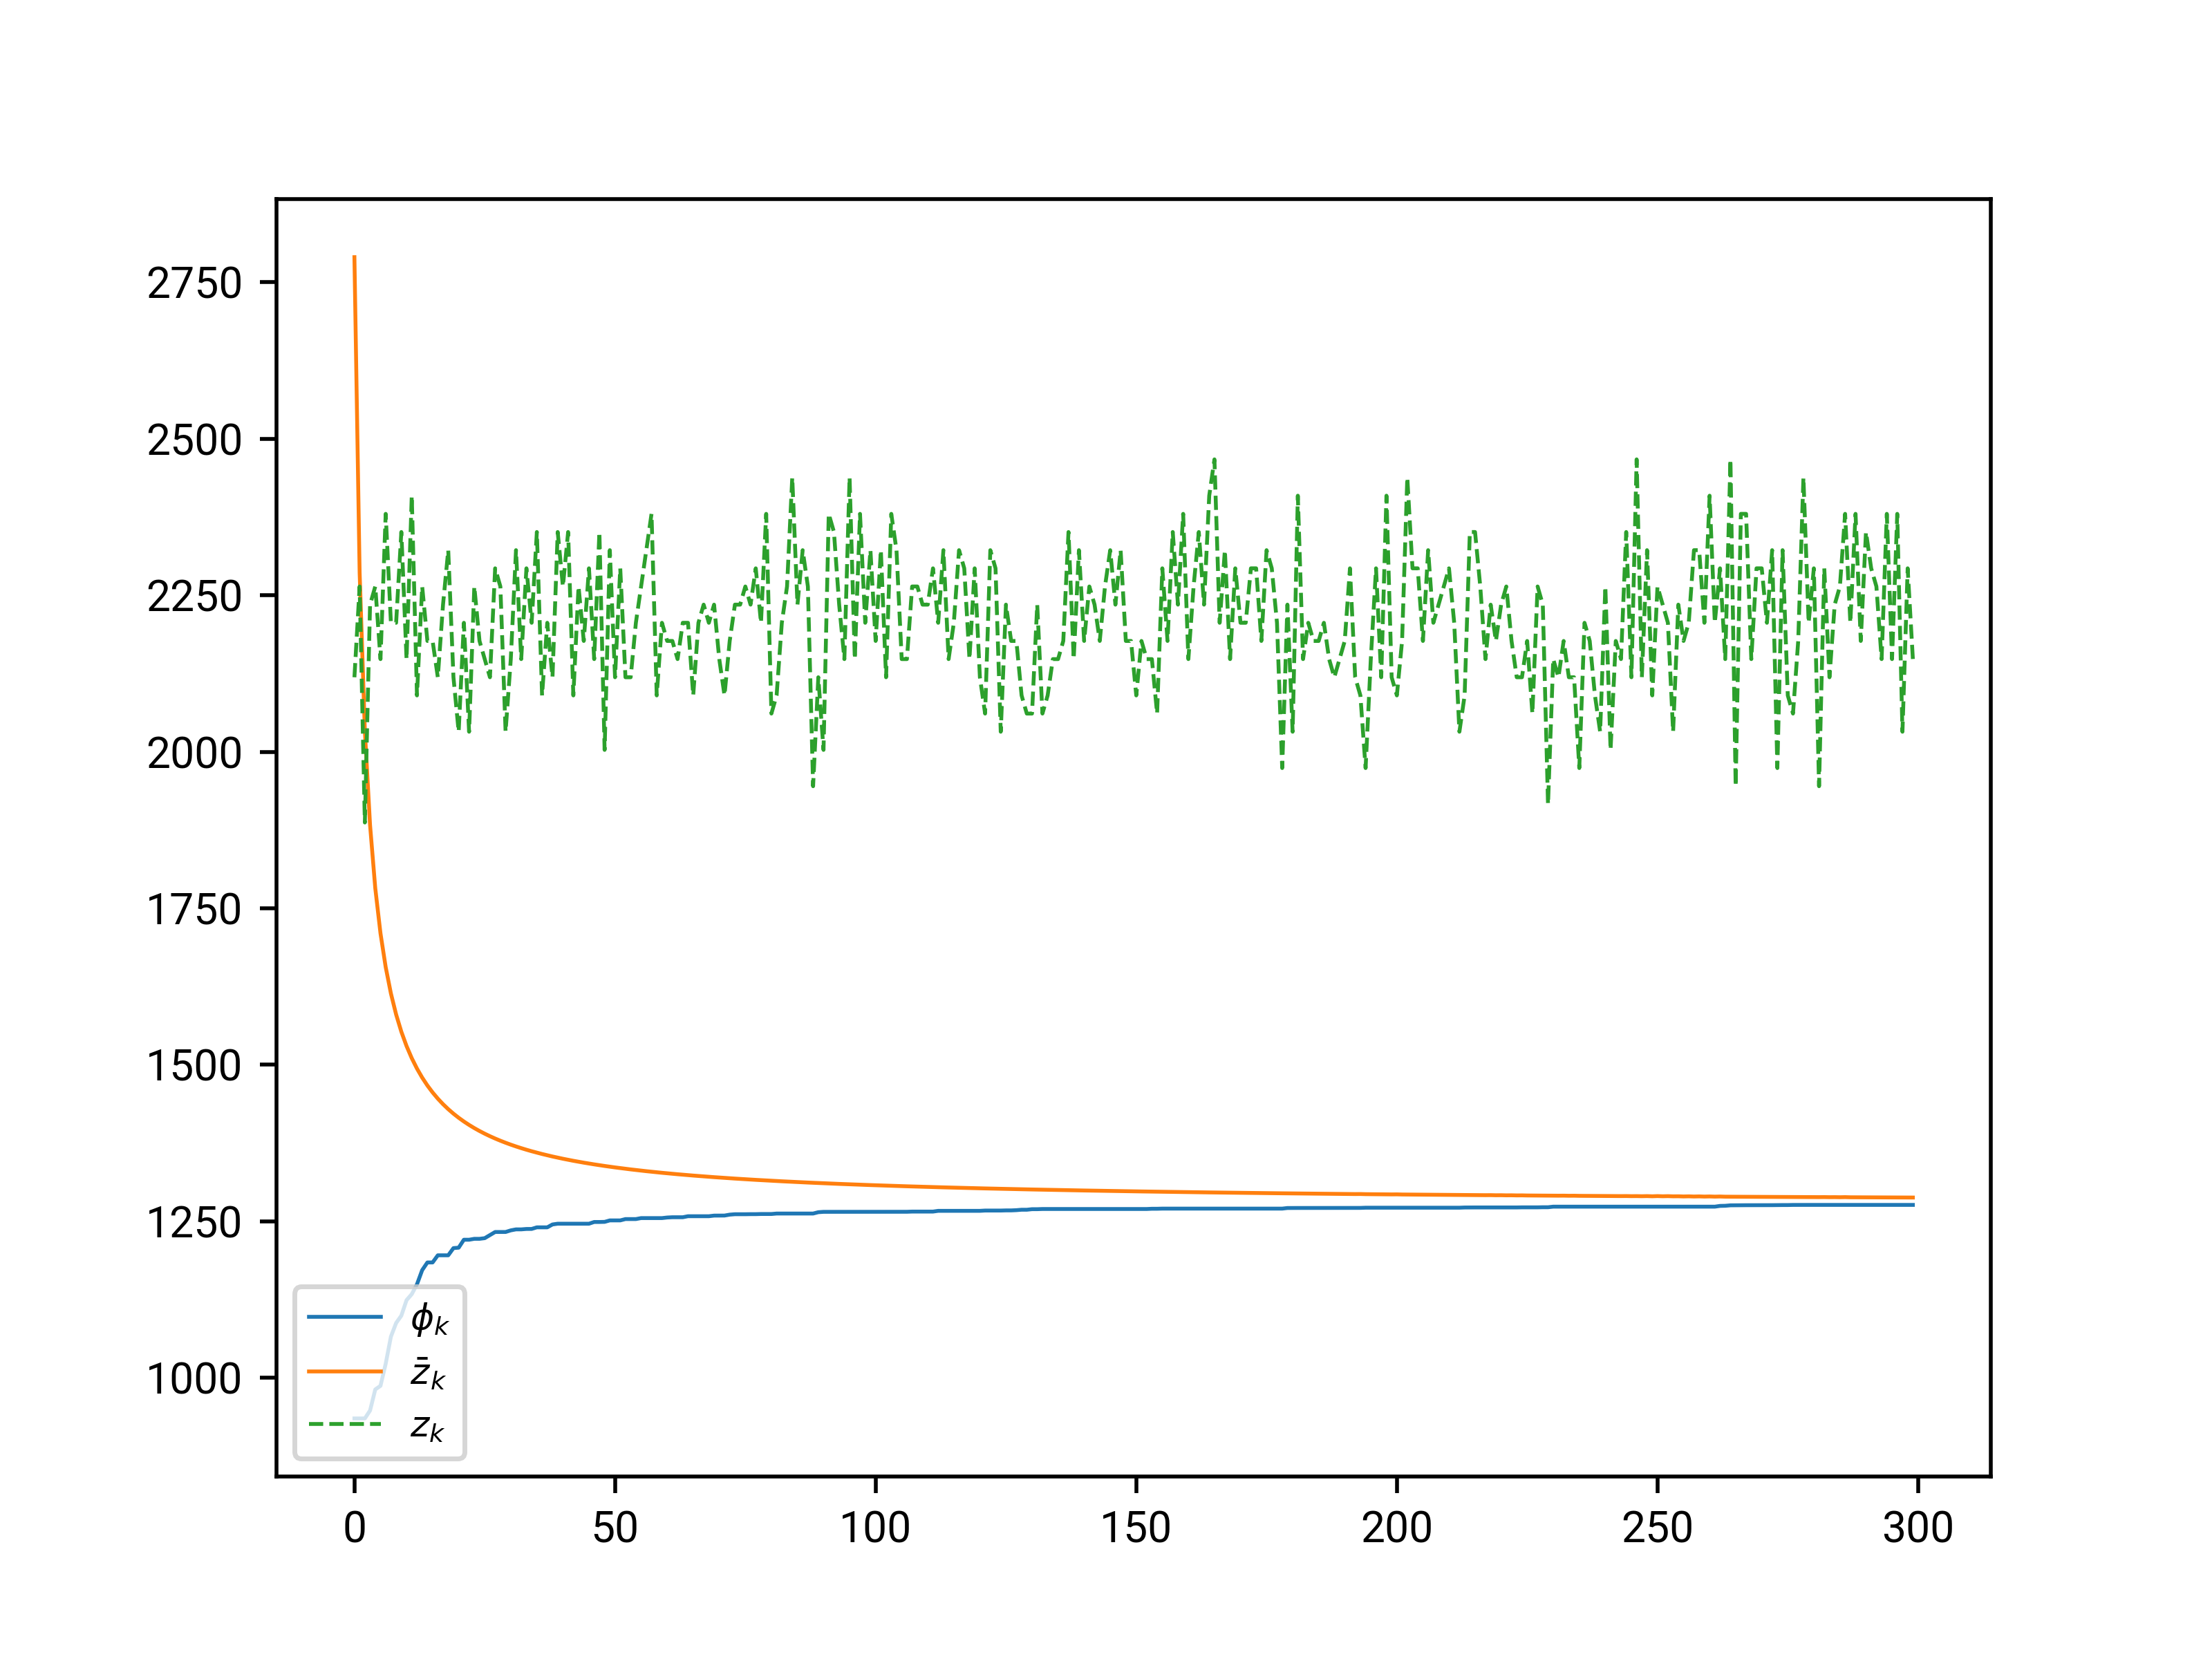
\includegraphics[width=.49\linewidth]{imgs/conv_0_normal_sg_5_80.png}
    }
    \subfloat[][Convex subgradient method using \(d_k\)]{
      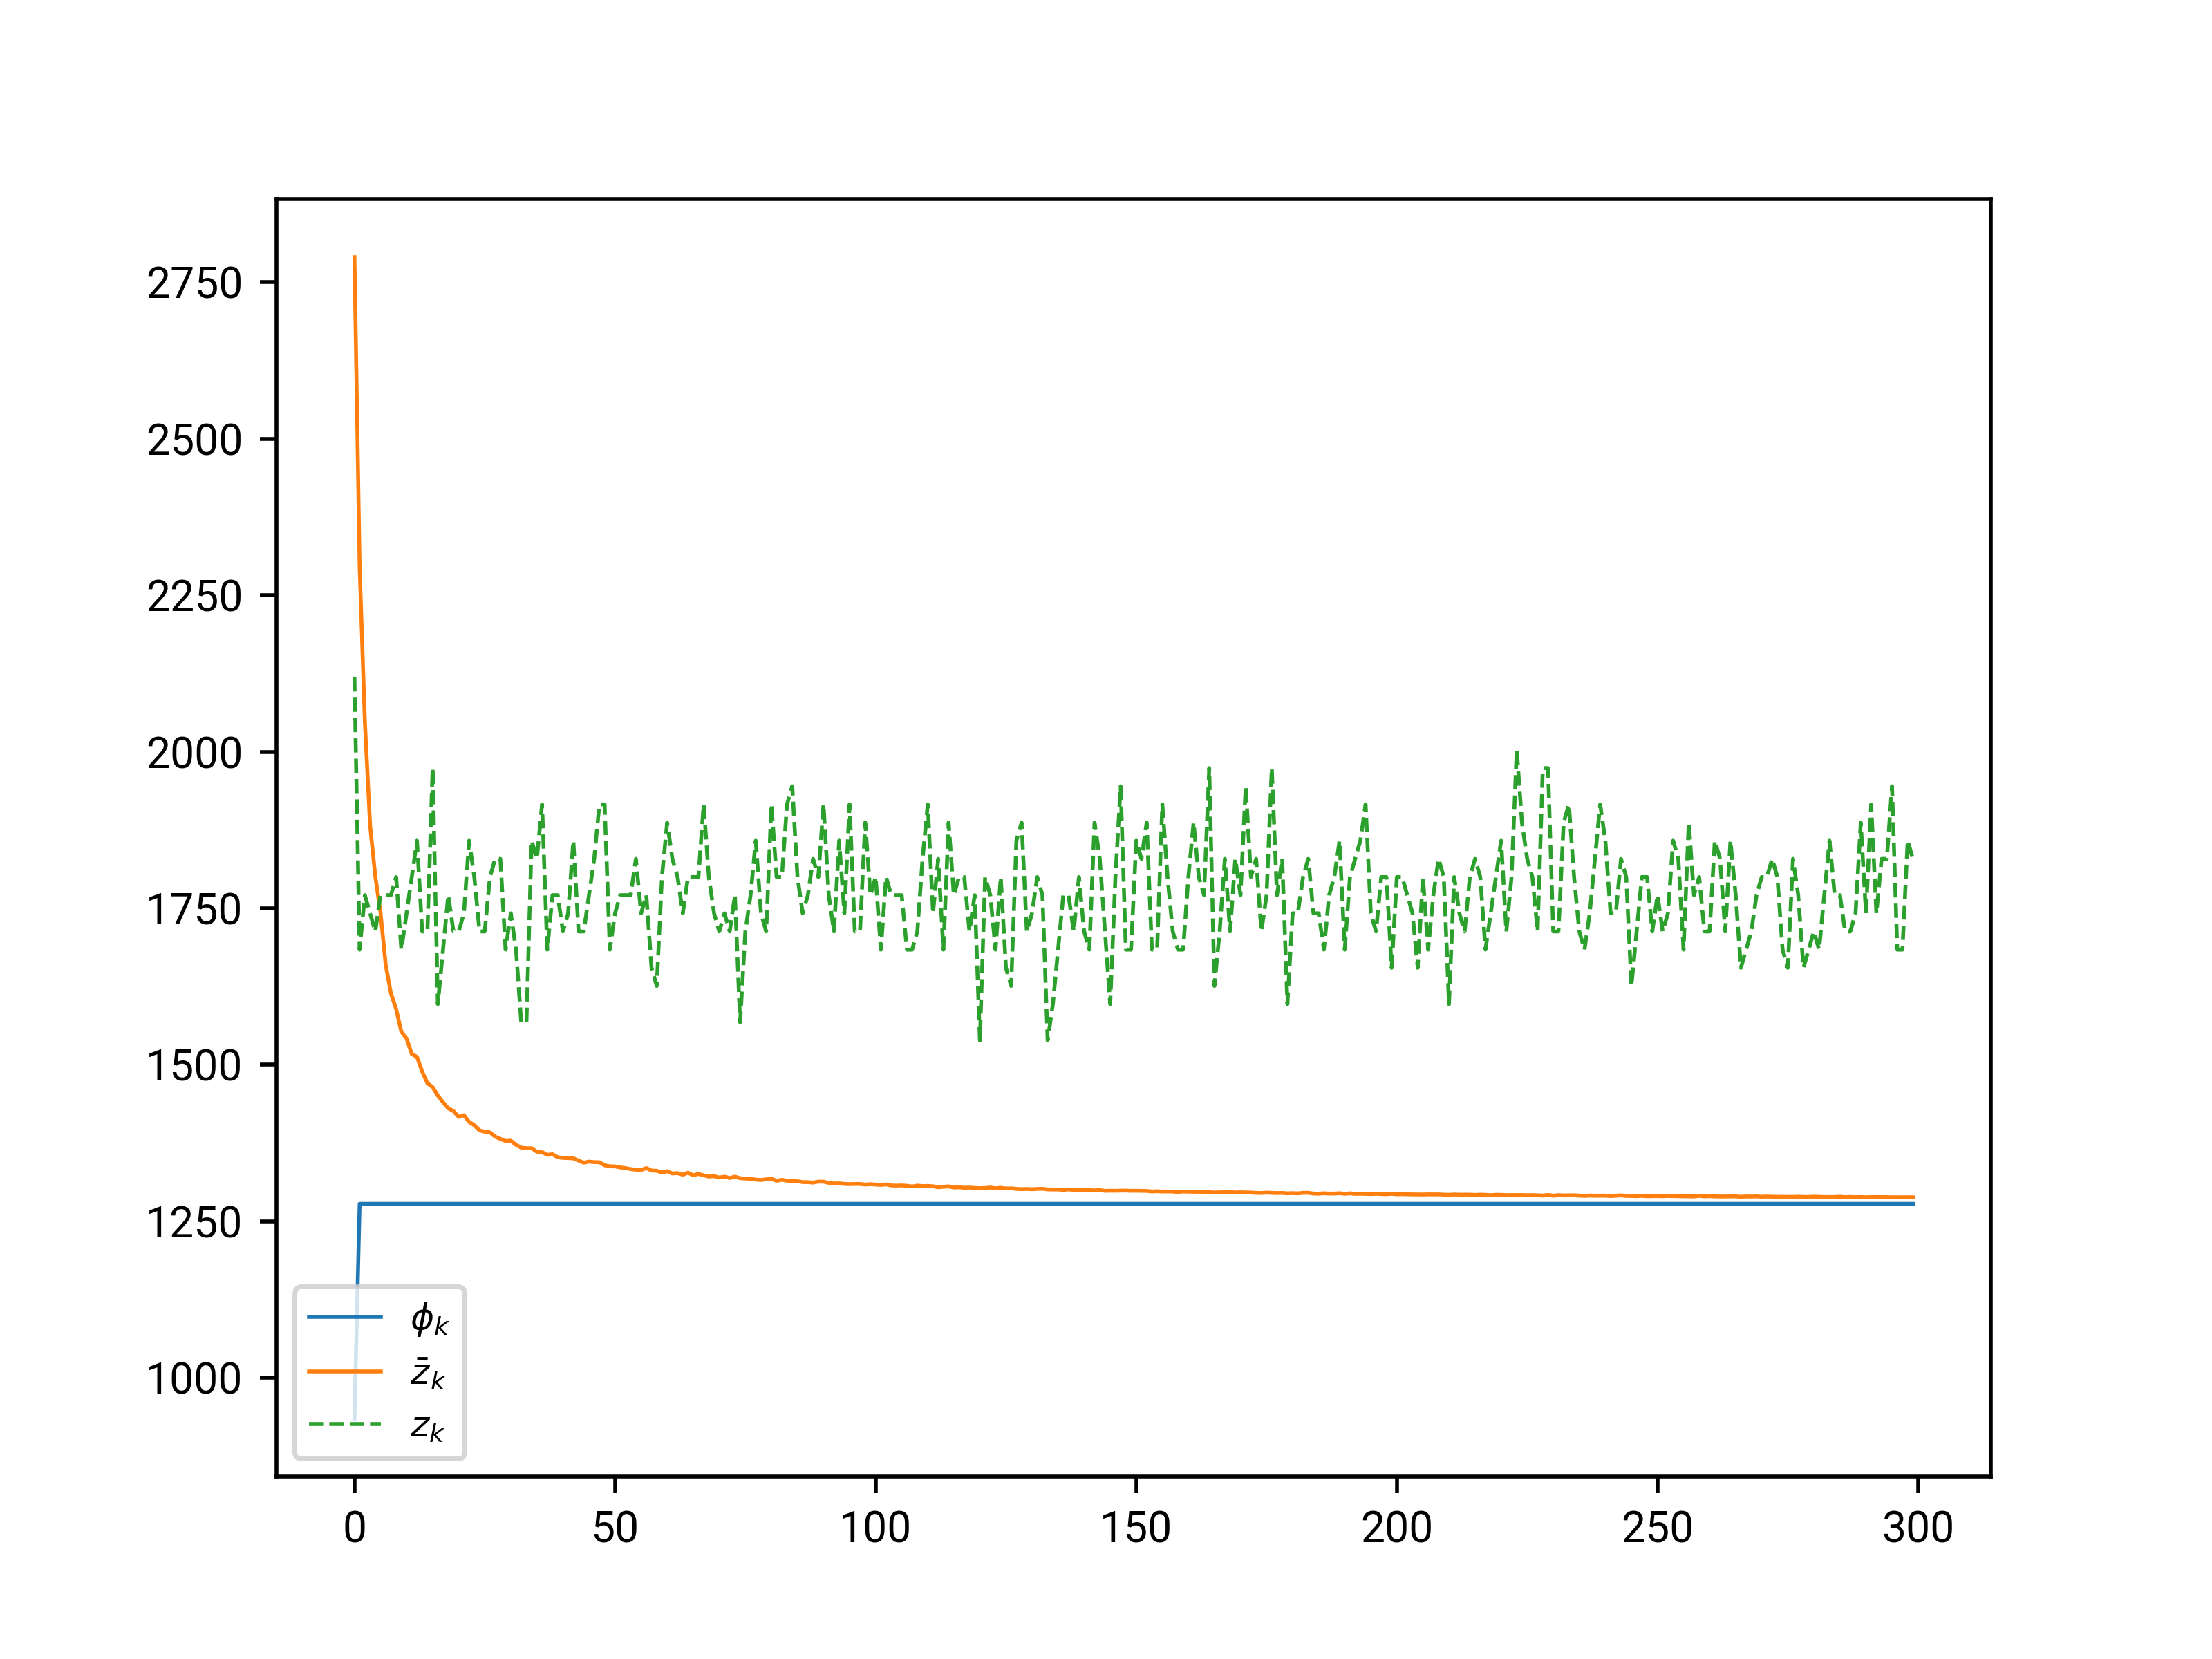
\includegraphics[width=.49\linewidth]{imgs/conv_0_convex_sg_5_80.png}
    }
  \end{figure}
\end{frame}
\end{document}
